\newpage
\begin{question}
Prove that $\sum_{j=1}^n j(j+1)(j+2) \cdots(j+k-1)=n(n+1)$ $(n+2) \cdots(n+k) /(k+1)$ for all positive integers $k$ and n. [Hint: Use a technique from Exercise 33]


\begin{figure}[h!]
    \centering
    \fbox{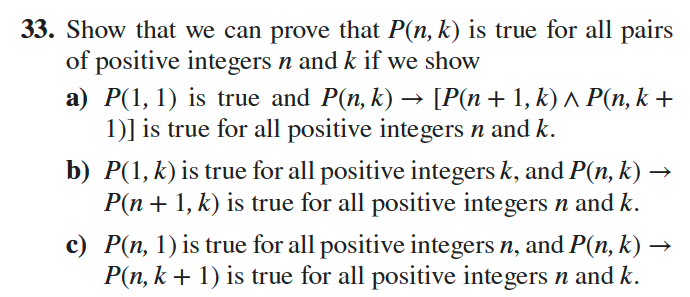
\includegraphics[width=0.5\linewidth]{questions/Exer33.png}}
\end{figure}

\end{question}

\par\noindent\rule{\textwidth}{0.5pt}

\subsubsection*{Solutions}

\begin{proof}
    Let $P(n, k)$ be the statement $\sum_{j=1}^n j(j+1)(j+2) \cdots(j+k-1)=n(n+1)$ $(n+2) \cdots(n+k) /(k+1)$ for all positive integers $k$ and n. We will prove that $P(n, k)$ is true for all pairs of positive integers $n$ and $k$ by induction on $n$ and $k$ followinng the step $b$ of Exercise 33.\\
    \textbf{Base Case:} \\
    $P(1, k) \Longleftrightarrow \sum_{j=1}^1 j(j+1)(j+2) \cdots(j+k-1) = 1(1+1)(1+2) \cdots(1+k-1) = 1 = 1(1+1)(1+2) \cdots(1+k)/(k+1)$ is true for all positive integer $k$.\\
    \begin{align*}
        P(n+1, k) \Longleftrightarrow & \sum_{j=1}^{n+1} j(j+1)(j+2) \cdots(j+k-1) \\
        = &\sum_{j=1}^{n} j(j+1)(j+2) \cdots(j+k-1) + (n+1)(n+2) \cdots(n+k)\\
        = & \frac {n(n+1) \cdots(n+k)} {k+1} + (n+1)(n+2) \cdots(n+k) & \because \text{$P(n, k)$ is true}\\
        = & \frac {n(n+1) \cdots(n+k) + (n+1)(n+2) \cdots(n+k)(k+1)} {k+1}\\
        = & \frac {(n+1)(n+2) \cdots(n+k)(n+k+1)} {k+1} & \text{So, $P(n+1, k)$ is true}
    \end{align*}
    Therefore, by induction, $P(n, k)$ is true for all positive integers $n$ and $k$.
\end{proof}